\documentclass[a4paper, 11pt]{article}
\usepackage{tbagrelstandard}
\usepackage{concretefull}
\usepackage{listingsstylebluesky}
\usepackage{float}

\newcommand{\HRule}{\rule{\linewidth}{0.5mm}}

\newcommand{\liu}{\sf{Light It Up!}}
\newcommand{\isn}{\sc{isn}}
\newcommand{\icn}{\sc{icn}}
\newcommand{\py}{\sf{Python}}
\newcommand{\pygtk}{\sf{pyGTK}}
\newcommand{\pygame}{\sf{Pygame}}
\newcommand{\nomcarte}{\sf{Adafruit CircuitPython}}
\newcommand{\led}{\sc{led}}
\newcommand{\rvb}{\sc{rvb}}
\newcommand{\gimp}{\sf{GIMP}}

\setlength{\parskip}{0.5\baselineskip}

\begin{document}

\thispagestyle{empty}
\begin{titlepage}

\center{}

%------------------------------------------------------------------------------
% HEADING SECTIONS
%------------------------------------------------------------------------------

\hspace{0pt}
\vfill{}

\textsc{\Large Lycée Arthur Varoquaux}\\[1.2cm]

%------------------------------------------------------------------------------
% TITLE SECTION
%------------------------------------------------------------------------------

\HRule \\[0.4cm]
{ \huge \bfseries Projet ISN}\\
\HRule \\[1.3cm]

%------------------------------------------------------------------------------
% AUTHOR SECTION
%------------------------------------------------------------------------------

\begin{minipage}[t]{0.38\textwidth}
\begin{flushleft} \large
\mbox{}\\
\begin{tabular}{ll}
\emph{Auteurs~:}\quad & Marie \sc{BAGREL}\\
&Célian \sc{BECQUES}
\end{tabular}

\end{flushleft}
\end{minipage}
\hfill
\begin{minipage}[t]{0.58\textwidth}
\begin{flushright} \large
\mbox{}\\
\begin{tabular}{ll}
\emph{Enseignants~:}\quad & M. \sc{Rougeaux}\\
&M. \sc{Thomas}\\
&M. \sc{Maginot}
\end{tabular}
\end{flushright}
\end{minipage}\\[1.5cm]

%------------------------------------------------------------------------------
% DATE SECTION
%------------------------------------------------------------------------------

{\large Année 2018 - 2019}\\[1.2cm]

%------------------------------------------------------------------------------
% LOGO SECTION
%------------------------------------------------------------------------------


\includegraphics[width=6cm]{etablissement.png}

\vfill{}
\end{titlepage}
\clearpage{}

Nous allons vous présenter le programme \liu{} qui constitue notre projet de fin d'année dans le cadre de la spécialité \isn{} de terminale S.
Ce projet a été mené à bien par Marie \sc{Bagrel} et Célian \sc{Becques}, tous deux élèves de terminale S-1. Il est donc le fruit de nombreuses heures de travail venant de chaque membre du groupe.

\section*{Création du groupe}

Nous n'avons pas eu beaucoup de problèmes pour former notre binôme. Effectivement, nous avons tous deux, ainsi que quelques autres élèves de notre classe de première, suivis l'option facultative \icn{} qui nous a permis d'acquérir déjà certaines bases dans la programmation en \py{} ainsi qu'avec des cartes programmables. Nous avions donc déjà décidé l'année dernière de faire la spécialité \isn{}. Cette année, étant dans le même groupe de spécialité, et étant aussi en très bons termes, le choix de faire équipe pour le projet final nous est apparu comme une évidence. De plus, étant tous les deux intéressés par des aspects de la programmation, nous avons pensé qu'il serait peut-être plus facile de se répartir efficacement le travail. Malgré les sollicitations de certains de nos camarades, nous avons préféré demeurer en binôme pour une meilleure organisation, notamment pour le travail en dehors des deux heures hebdomadaires d'\isn{}.

\section*{Origine du projet}

Une fois le binôme constitué, nous avons très longuement cherché une idée de projet qui puisse nous satisfaire tous les deux. Nous avons, pour arriver à une idée adaptée et réalisable, fait une liste des différentes contraintes qu'il fallait remplir selon nous pour mener à bien le projet. Nous voulions un programme qui puisse contenir une partie programmation pure avec le langage de programmation \py{}, puisque c'est celui qui nous avait été enseigné tous le long de notre option l'année passée. Mais d'un autre côté, nous voulions un projet qui puisse aussi contenir un composant externe à l'ordinateur tel qu'un potentiomètre, une \led{}, une photorésistance\ldots{} On en a donc déduit qu'il fallait utiliser une carte programmable, et nous avons choisit le circuit \nomcarte{} sachant que nous avions déjà pu découvrir son fonctionnement global en début d'année.

Avec ces informations, nous avons donc cherché une idée de programme, plutôt orientée vers un jeu. C'est Célian qui proposa une idée pouvant répondre aux principales contraintes : \emph{un parc d'attraction miniature}. Pour cela, il eut l'idée de réaliser différents stands de jeu tels qu'un tir sur une cible, une pêche aux canards\ldots{} Il pensait faire intervenir un robot monté sur un chariot pour permettre le jeu. Même si l'idée nous convenait à tous les deux, lorsque nous en avons parlé aux professeurs la semaine suivante, ils nous on fait réaliser que nous avions oublié une contrainte essentielle : le temps. En effet, notre projet bien qu'attrayant, était excessivement ambitieux compte-tenu du temps disponible pour le réaliser : 3 mois. Par conséquent, cette échéance nous à fait revenir au point mort : nous n'avions toujours pas de projet. Après deux semaines de recherches, c'est finalement Marie qui a apporté une idée de projet adaptée : un jeu de mémorisation de séquence de couleurs, avec une interface graphique sur l'ordinateur connecté à la carte. Ce projet était à lui seul assez ambitieux pour nous occuper durant les 3 mois restant.

\section*{Le détail du projet}

Le projet a donc enfin été trouvé et peu de temps après, nous nous sommes rendus compte que ce jeu de mémorisation existait déjà en version commercialisable sous le nom de \emph{Simon} depuis 1978. Dans ce jeu, une séquence de couleurs s'allume sur un boîtier et le joueur doit la reproduire par la suite à l'aide des boutons correspondants sans faire d'erreur malgré la difficuté croissante des niveaux et le chronomètre qui défile. Nous nous sommes donc appuyé de ce principe pour en apporter des variantes : nous voulions, en plus de la séquence aléatoire de \led{}s qui s'affiche, avoir la possibilité de modifier la couleur de chaque \led{} pour y apporter plus de confusion. Nous voulions également faire deux modes de jeu : le mode solo dans un premier temps puis un mode multijoueur dans un second. Concernant l'interface graphique sur l'ordinateur, nous avons directement pensé à \pygtk{}, qui aurait permi de réaliser facilement les nombreux boutons et les différentes fenêtres.

Une fois le projet déjà bien déterminé, nous l'avons exposé à nos professeurs d'\isn{} pour ainsi obtenir leur avis mais aussi pour savoir s'ils disposaient du matériel dont nous avions besoin. Ayant tout le matériel nécessaire, les professeurs ont approuvé notre projet mais nous ont dit de nous diriger vers une interface \pygame{} plutôt que \pygtk{}. Nous avons été un peu déstabilisé d'apprendre que nous allions devoir utiliser \pygame{}, car même si les professeurs nous ont assuré qu'avec ce module, il serait plus facile de mener à bien notre projet, nous avons surtout vu par la suite toutes les inconvénients liés à cette librairie comme l'absence de réel boutons, la nécessité d'une rafraichissement manuel de l'interface\ldots{}. Comme nous n'avions qu'une année d'expérience en programmation, nous leur avons fait confiance. Nous nous sommes donc enfin lancés dans notre projet. Vu que nous nous connaissions bien, nous avions chacun une idée claire de la distribution du travail : Célian allait réaliser l'interface graphique sous \pygame{}, tandis que Marie allait écrire le code pour la carte \nomcarte{}, pour contrôler les \led{}s et les boutons.

Une semaine plus tard, les professeurs nous on remis les composants utiles pour notre projet ils nous ont monté le tout sur une plaque. Voici les principaux composants du système :

\begin{center}
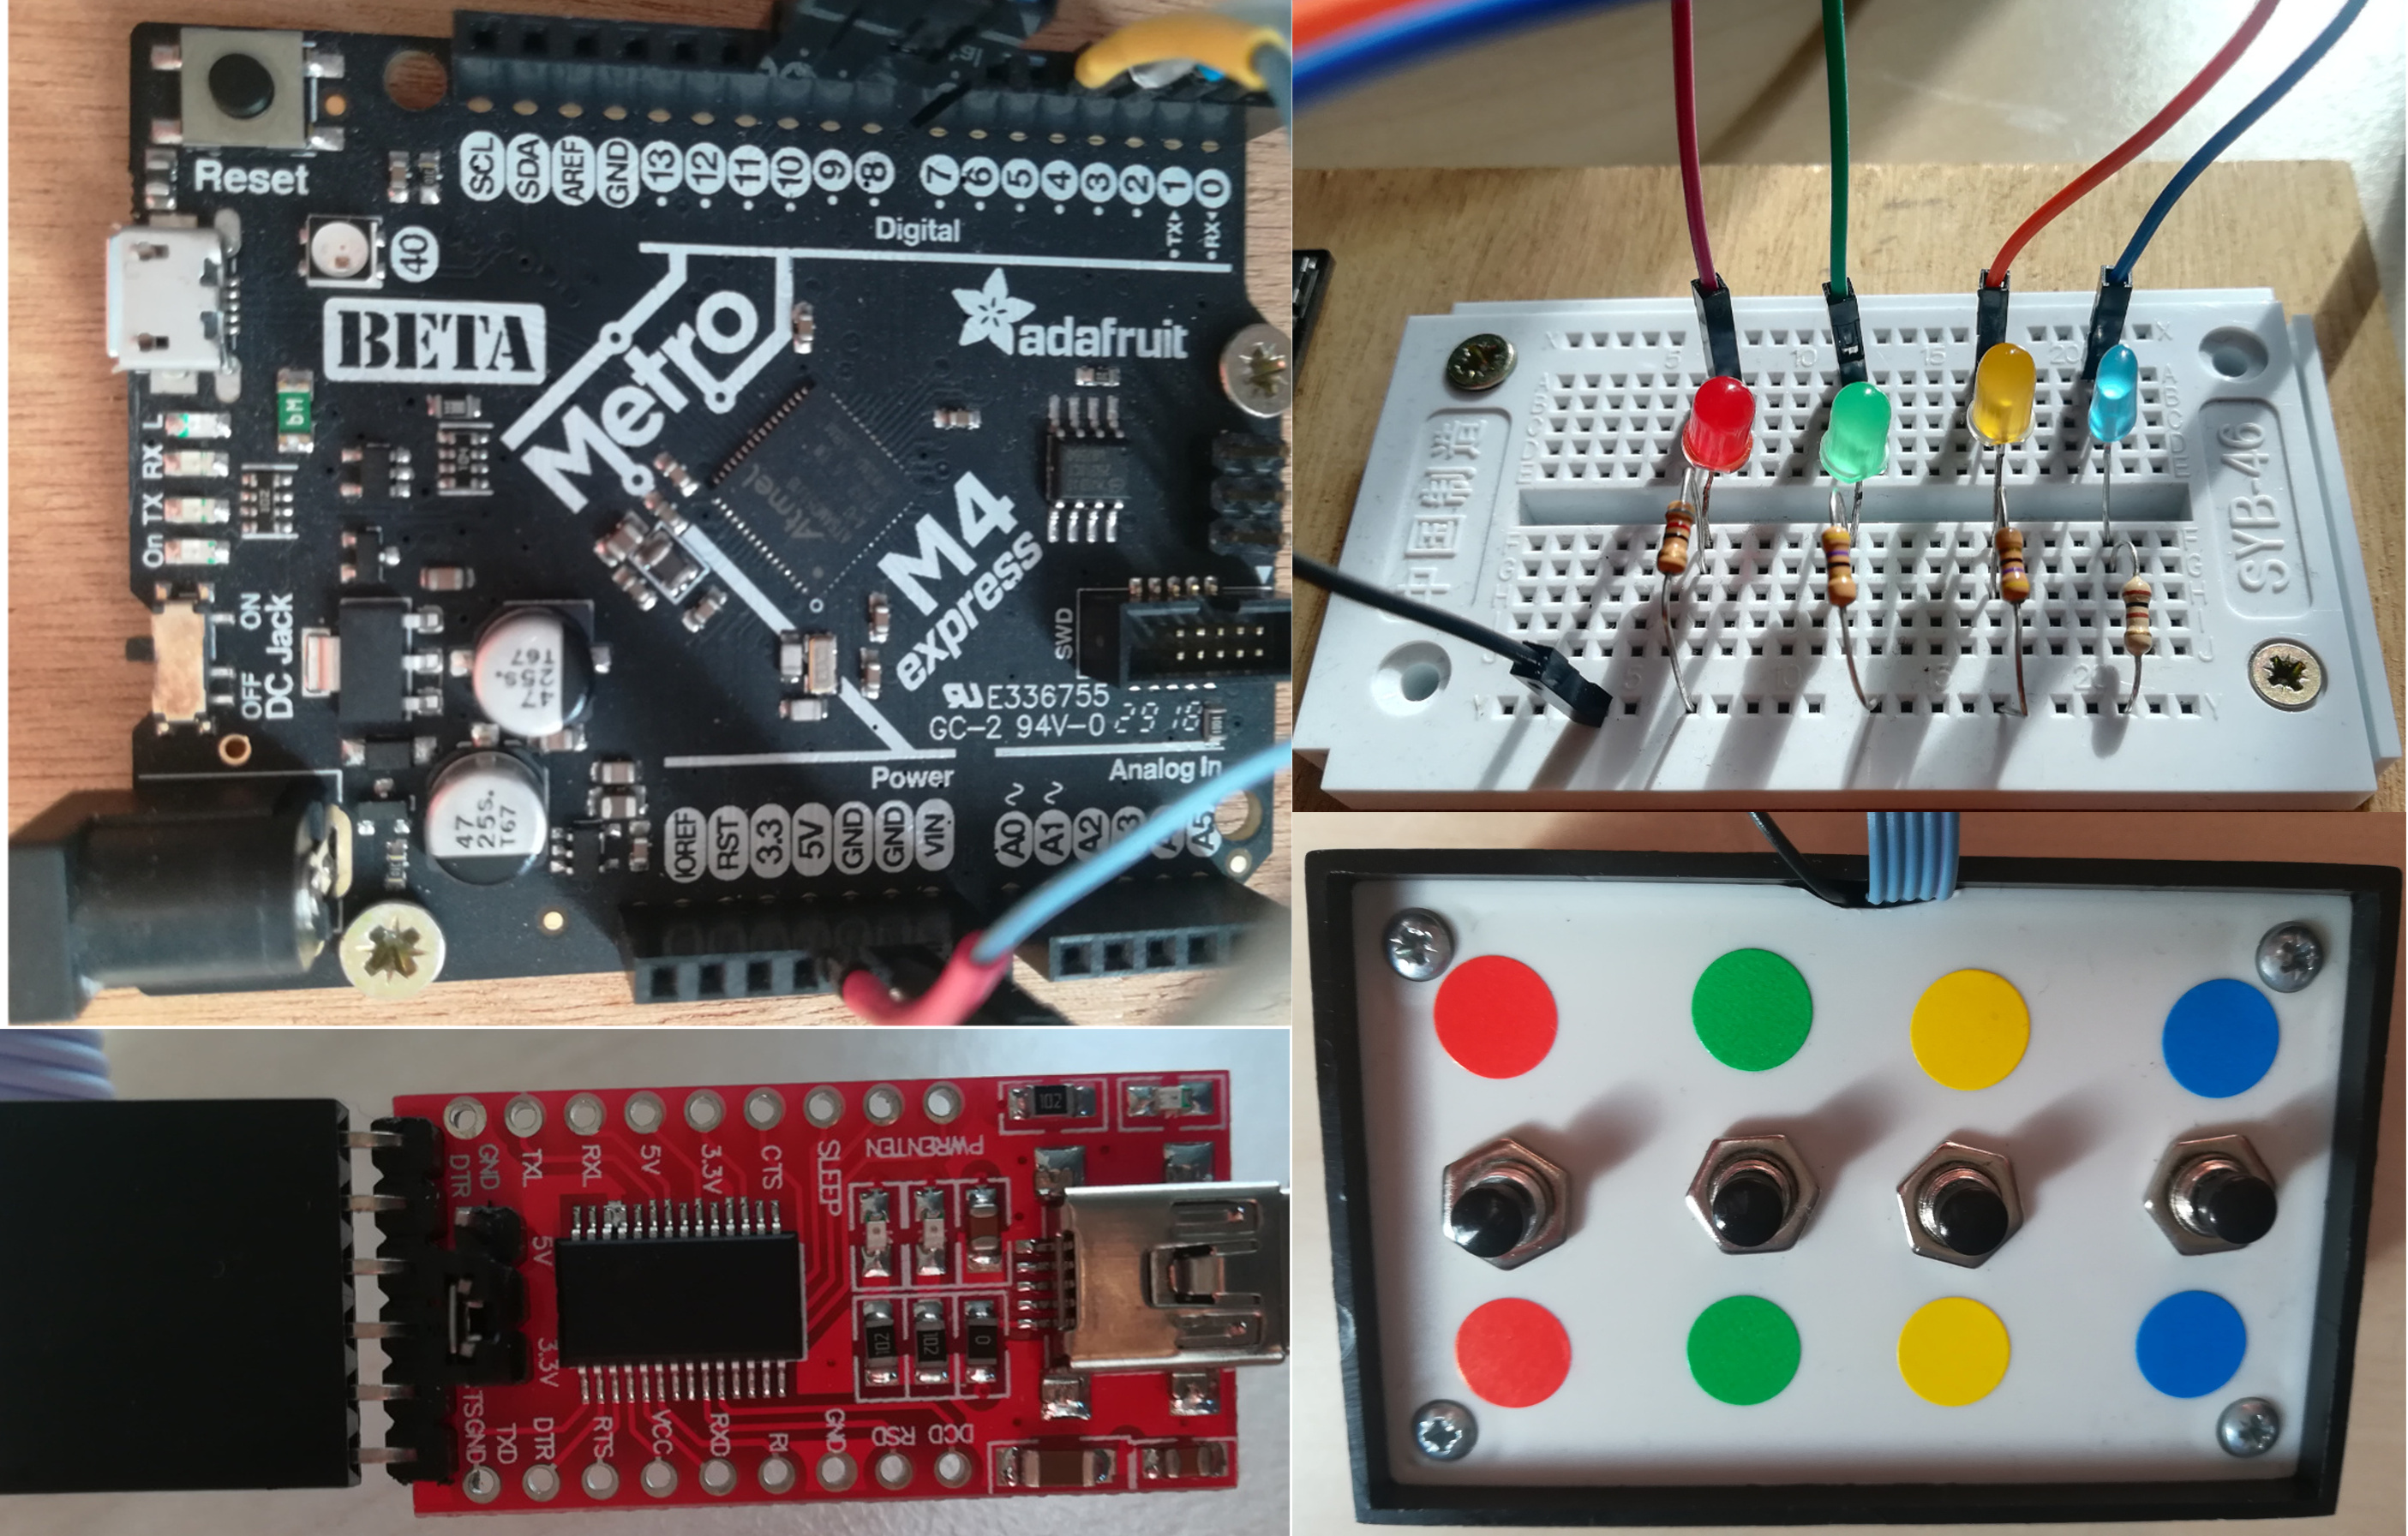
\includegraphics[width = 12 cm]{projet.jpg}
\captionof{figure}{la carte , les leds, le composant de communication et le boitier avec les boutons}
\end{center}

\section*{Les difficultés rencontrées}

Nous avons, lors de notre projet, rencontré de nombreuses difficultés que nous avons surmontées ou contournées.

La principale difficulté fut de maîtriser l'état des boutons à presser pour permettre de reproduire la séquence de \led{}. En effet, ces boutons étaient initialement branchés sur les entrées analogiques de la carte, puisque les \led{} \rvb{} occupaient tous les ports numériques (3 ports par \led{}), ceci afin de permettre d'obtenir toutes les couleurs désirées. Marie a donc essayé de faire fonctionner les boutons à de nombreuses reprises, mais malgré un programme sans erreur apparente, des pressions sur deux boutons différents étaient parfois détectées alors qu'un seul était pressé. Même avec de l'aide extérieure, le problème n'a pas pu être résolu. Nous avons donc décidé de retirer les \led{}s \rvb{} de notre programme pour les remplacer par des \led{}s classiques : rouge, verte, jaune et bleue. Ce changement a permi de libérer des ports numériques pour ainsi faire fonctionner facilement les boutons. Suite à ce changement conséquent, nous sommes partis sur des bases plus sûres pour la suite de notre projet.

Nous avons aussi pu rencontrer un problème concernant les boutons qui a été résolu grâce à un changement dans le programme de la carte. En effet, lorsque que nous appuyions sur les boutons correspondant à la séquence allumée, nous avions parfois des erreurs indiquant que la séquence reproduite n'était pas identique, alors qu'elle aurait du l'être. Nous nous sommes rendus compte que cela arrivait lorsqu'une \led{} clignotait deux fois de suite et nous en avons déduit que la double pression du bouton n'était pas prise en compte ou mal interprétée. Nous avons donc décidé, pour pallier ce problème, d'empêcher une \led{} de s'allumer deux fois d'affilée dans une même séquence. Nous avons donc du modifier de façon conséquente notre programme. La fonction ci-dessous a été modifiée~:

\begin{lstlisting}[language=Python, float=H, caption=Fonction \tt{alea\_sequence} (avant)]
def alea_sequence(nombre_led_a_allumer):
    leds_a_allumer = []
    for led in range((nombre_led_a_allumer - 1)):
        pos = random.randint(0, 3)
        leds_a_allumer.append(pos)
    return leds_a_allumer
\end{lstlisting}

pour en faire deux distinctes en évitant la possibilité d'un rebond~:

\begin{lstlisting}[language=Python, float=H, caption=Fonctions \tt{alea\_led} et \tt{alea\_sequence} (après)]
def alea_led(derniere_pos):
    liste_alea_tirage = [[1, 2, 3], [0, 2, 3], [0, 1, 3], [0, 1, 2]]
    led_choisie = random.choice(liste_alea_tirage[derniere_pos])
    return led_choisie

def alea_sequence(nombre_led_a_allumer):
    leds_a_allumer = []
    derniere_pos = random.randint(0, 3)
    leds_a_allumer.append(derniere_pos)
    for led in range((nombre_led_a_allumer - 1)):
        derniere_pos = alea_led(derniere_pos)
        leds_a_allumer.append(derniere_pos)
    return leds_a_allumer
\end{lstlisting}

Ainsi, avec la fonction \verb=alea_led=, on peut tirer une position aléatoire de \led{} en tenant compte de la précédente et avec la fonction \verb=alea_sequence=, on peut générer une séquence aléatoire en utilisant la précédente fonction.

Un autre problème que nous avions déjà vu venir nous est apparu : le problème de création des boutons dans l'interface du jeu sur \pygame{}. Effectivement, nous n'avons pas la possibilité de créer des boutons à part entière sur \pygame{}, et cela a été vraiment handicapant. Nous avons après de nombreuses recherches trouvé une solution pour contourner le problème : nous avons créé des images qui représentaient des boutons puis, grâce aux coordonnées de la souris que nous pouvions récupérer, nous avons délimité des zones où le bouton était considéré comme cliqué, comme dans le code suivant~:

\begin{lstlisting}[language=Python, float=H, caption=Faux boutons sur \pygame{}]
for event in pygame.event.get():
    if event.type == QUIT:
        raise ToutQuitter("selection_mode_jeu")
    elif event.type == MOUSEBUTTONDOWN and event.button == CLIC_GAUCHE:
        # si on detecte l'evenement de clic gauche appuye de la souris
        pos_souris = pygame.mouse.get_pos()
        x_souris = pos_souris[0]
        y_souris = pos_souris[1]
        if 60 < x_souris < 360 and 320 < y_souris < 410:
            # le bouton solo est considere comme selectionne
            return SINGLEPLAYER
        elif 440 < x_souris < 740 and 320 < y_souris < 410:
            # le bouton deux joueurs est considere comme selectionne
            return MULTIPLAYER
\end{lstlisting}

Nous avons pu ainsi contourner notre problème.

Un dernier problème important lié à l'interface est finalement apparu : nous ne pouvions pas faire de zones de saisie de texte directement sur \pygame{}. Nous voulions pourtant pouvoir saisir le nom des joueurs dans le menu principal. Nous avions, au départ, utilisé la console \py{} pour saisir les noms tout en ayant l'espoir de trouver une solution pour les saisir directement. Nous avons là encore trouvé une façon détournée d'afficher les noms des joueurs pendant la saisie. Nous avons créé un dictionnaire donnant les correspondances entre les événements liés aux touches du clavier de \pygame{} et lesdites lettres. Nous avons lié cela à une liste contenant les lettres tapées au fur et à mesure de la saisie par le joueur :

\begin{lstlisting}[language=Python, float=H, caption=Saisie du nom du joueur]
CORRESPONDANCE_CLAVIER = {
    K_a: "a", K_b: "b", K_c: "c", K_d: "d", K_e: "e", K_f: "f", K_g: "g",
    K_h: "h", K_i: "i", K_j: "j", K_k: "k", K_l: "l", K_m: "m", K_n: "n",
    K_o: "o", K_p: "p", K_q: "q", K_r: "r", K_s: "s", K_t: "t", K_u: "u",
    K_v: "v", K_w: "w", K_x: "x", K_y: "y", K_z: "z"
}

nom_joueur = ""

for event in pygame.event.get():
    if event.type == QUIT:
        raise ToutQuitter("avant_partie_un_joueur")
    elif event.type == KEYDOWN:
        if event.key in CORRESPONDANCE_CLAVIER and saisie_en_cours:
            nom_joueur += CORRESPONDANCE_CLAVIER[event.key]
            nom_joueur = nom_joueur.title()
        if event.key == K_BACKSPACE and saisie_en_cours:
            nom_joueur = nom_joueur[: -1]
        if event.key == K_SPACE and saisie_en_cours:
            nom_joueur = nom_joueur + " "
\end{lstlisting}

Durant toute la création de l'interface, nous avons cherché à déterminer les coordonnées à utiliser pour que les éléments de notre interface soient centrés. Voyant qu'avec de simples feuilles de papier et une règle, nous peinions à déterminer la position de chaque élément, nous avons cherché un logiciel ou site internet pouvant nous aider. Après quelques recherches, nous avons choisi d'utiliser un site internet permettant de déterminer les tailles et les coordonnées des objets composant notre interface : \href{https://wireframe.cc/}{\tt{wireframe.cc}}, qui nous a été d'une grande aide~!

Nous avons aussi porté attention aux droits des images qui composaient notre programme. Effectivement, nous avions au départ utilisé des images de boutons issues d'internet qui n'étaient pas libres de droit. Pour pallier ce problème, nous avons décidé de créer par nous même les boutons dont nous avions besoin grâce au logiciel de traitement d'images \gimp{}. Ce logiciel a permi de rendre les images de boutons plus réelles et fidèles à nos attentes, ainsi que de créer un logo pour notre jeu plutôt réussi. Tous les composants de notre programme sont par conséquent libres de droits. On peut d'ailleurs voir l'apparence de l'interface ci dessous:

\begin{center}
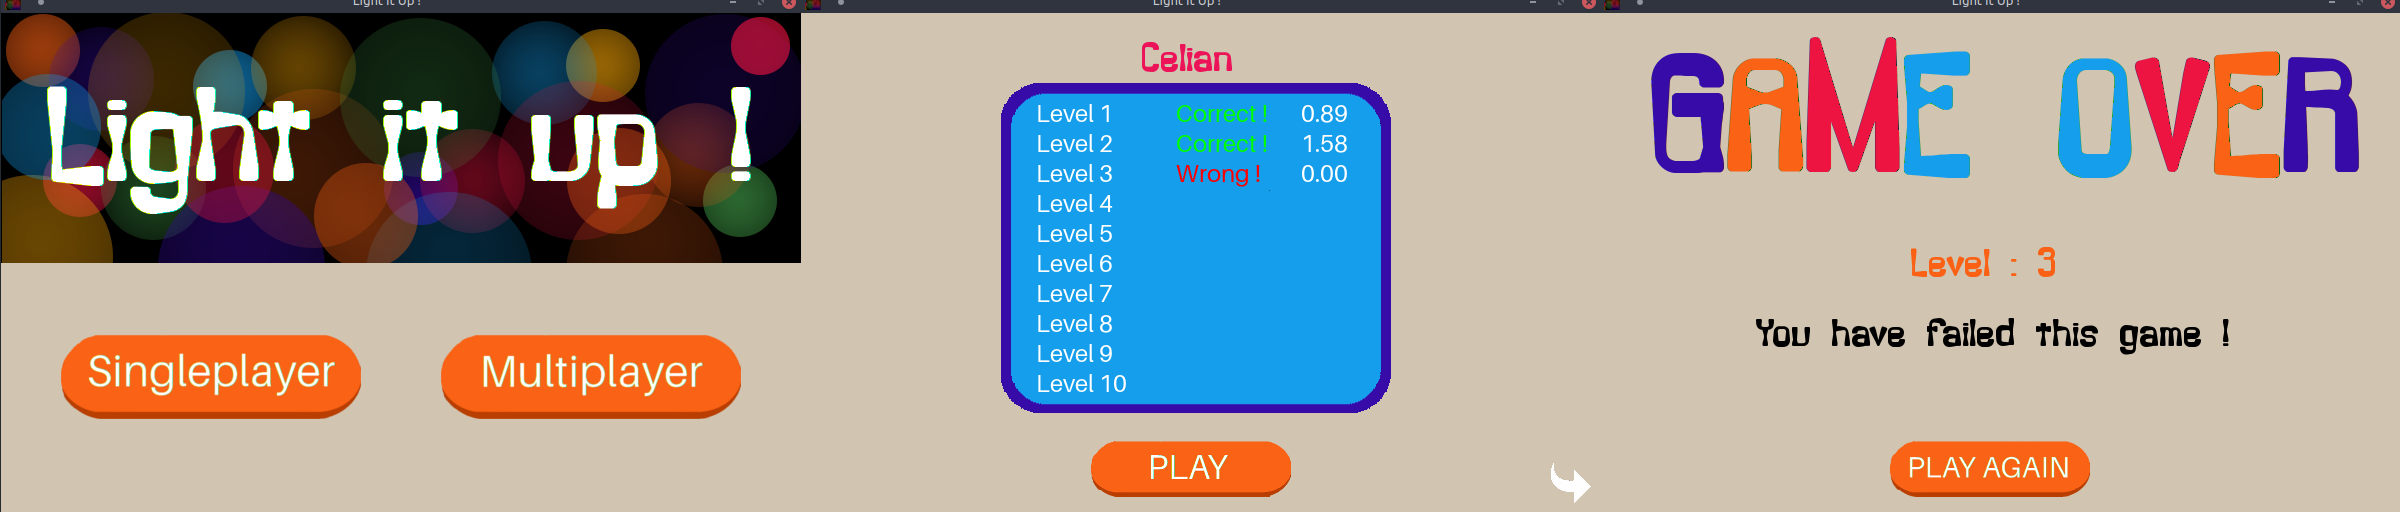
\includegraphics[width = 17cm]{interface.png}
\captionof{figure}{L'interface du mode solo}
\end{center}


On pourra conclure en disant que nous avons réussi à résoudre ou contourner nos problèmes mais un fut récurrent et nous ne sommes d'aileurs pas les seuls à l'avoir eu : la carte programmable est plutôt instable et par conséquent, de nombreuses difficultés sont apparues tout le long de notre projet. Du fichier main qui disparait ou qui est vidé par la carte, à la carte qui ``mange'' certaines lettres en passant par des reboot on justifiés, nous pouvons dire que cette carte nous en a fait voir de toutes les couleurs.

\section*{Ressentis personnels, expérience et amélioration}

\subsection*{Le mot de Marie}

Je suis très contente de la réalisation de ce projet. Ce dernier a nécessité un engagement permanent tout au long du dernier trimestre, ce qui, en prenant en compte les nombreuses autres épreuves, ne fut pas facile. Cependant, je suis contente que nous ayions réussi à le terminer dans les temps. J'ai été surprise de la difficulté de communication entre la carte et l'ordinateur, ce qui fut d'ailleurs la principale difficulté pour ma part. En effet, malgré un code juste, des erreurs aléatoires apparaissent sans raisons valables. Mais en général, je peux dire que le fruit de tout notre travail me satisfait. J'ai également apprécié travaillé en équipe et cela m'a d'ailleurs permis de voir qu'une division efficace du travail nous faisait gagner du temps. Avec Célian, nous n'avons pas eu de désaccord important durant la création du projet, mais au contraire, nous nous entraidions dans nos différentes parties. Je le remercie donc pour son travail et je suis d'ailleurs contente d'avoir pu réaliser ce projet en sa compagnie.
Si l'on devait apporter des améliorations à notre projet, je pense qu'on pourrait rajouter un bip sonore lorsque le joueur reproduit la séquence de \led{}s. De plus, un système de score pourrait aussi être réalisable. Enfin, si l'on veut augmenter le challenge, je pense que plus que six \led{}s sur la plaque au lieu de quatre serait un changement adéquat.
Enfin, si je devais porter un esprit critique sur notre projet, je dirais que nous avons eu du mal à décider ce que nous allions faire ce qui a réduit les délais déjà courts. De plus, les différentes épreuves autres que l'\isn{}, nous on limités dans nos ambitions. Si je devais refaire un projet comme celui-ci, je choisirais surement une autre librairie pour l'interface pour plus de facilité.

\subsection*{Le mot de Célian}

\section*{Remerciements}

Nous tenions à remercier pour ce projet, nos professeurs d'ISN, M. Rougeaux, M. Thomas et M. Maginot qui nous ont accompagné durant tous notre projet et qui ont su résoudre nos problèmes, mais aussi nous aiguiller dans nos choix et nous fournir également le matériel nécessaire. Ils nous ont permis également de découvrir la programmation durant toute l'année de façon passionnée.
Nous remercions également nos familles qui ont pu nous aider en testant le programme au cours de sa création pour détecter les points à améliorer, ou qui nous ont aidé pour le choix du nom du jeu, ou encore à relire ce dossier.

\section*{Contenu joint}

- le code complet constitué d'une partie interface graphique et le code de la carte programmable
- les images ou fichier nécessaires au bon fonctionnement du programme
- Ce dossier de présentation



\end{document}